\documentclass[aspectratio=169,11pt]{beamer}
\usepackage{luatexja}                % 日本語
\usepackage[haranoaji]{luatexja-preset} % 原ノ味フォント（標準同梱）
\usepackage{amsmath,amssymb,bm}
\usepackage{tikz}

\usetheme{Madrid}
\usecolortheme{seahorse}

\title{特異学習理論入門}
\author{Shiryu Nakano}
\date{\today}

\AtBeginSection[]{
  \begin{frame}{目次}
    \tableofcontents[currentsection]
  \end{frame}
}

\begin{document}
\frame{\titlepage}

\begin{frame}{目次}
  \tableofcontents
\end{frame}

\section{ベイズ推測の導入}

\begin{frame}{問題設定}
  N次元ユークリッド空間に${n}$個の点があるとする．
  $$x_i\in \mathbf{R}^{N}, (i = 1,2,...,n)$$
  これを以下のように書いて，*サンプル*と呼ぶ．
  $$x^n = (x_1,x_2,...,x_n) \in \mathbf{R}^{N} \dots \mathbf{R}^{N}$$
\end{frame}

\begin{frame}{道具立て}

  \item $q(x)$ : 真の分布
    \item $p(x \mid w)$ : 統計モデル（パラメータ $w \in W$）
    \item $\varphi(w)$ : 事前分布
\end{frame}

\begin{frame}{道具立て}

  \item $p(w|X^n)$ : 事後分布
  \item  $p(w|X^n) := \frac{\varphi(w)\prod_{i=1}^{N}p(x_i \mid w)}{Z_n(\beta)}
\end{frame}


\section{図の例}

\begin{frame}{図の挿入}
  \begin{figure}
    \centering
    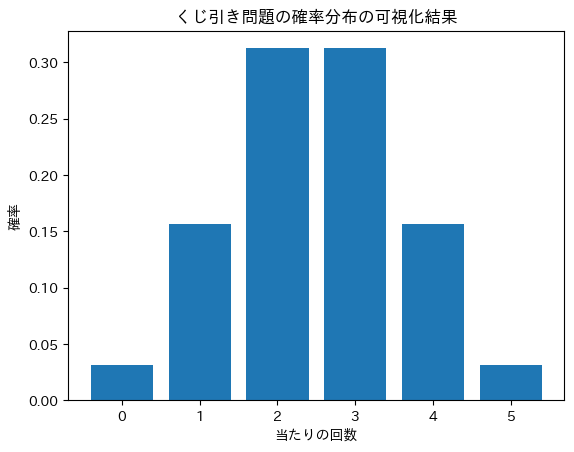
\includegraphics[width=0.7\linewidth,height=0.75\textheight,keepaspectratio]{figures/fig_1_1.png}
    \caption{サンプル図（fig\_1\_1）}
  \end{figure}
\end{frame}

\section{まとめ}

\begin{frame}{まとめ}
  \begin{itemize}
    \item 特異モデルでは古典的漸近論が破綻
    \item 実対数閾値 $\lambda$ が汎化誤差の主要項を決める
  \end{itemize}
\end{frame}

\section{テスト}
\begin{frame}{図と説明}
  \begin{columns}[T]                       % T = 上揃え
    \begin{column}{0.55\textwidth}         % 左カラム 55%
      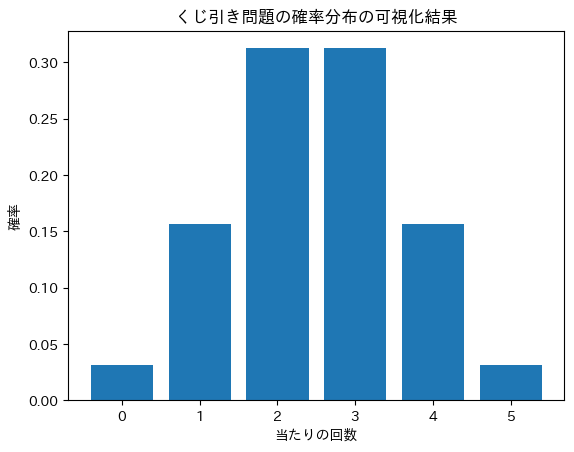
\includegraphics[width=\linewidth,
        height=0.75\textheight,keepaspectratio]{figures/fig_1_1.png}
    \end{column}
    \begin{column}{0.45\textwidth}         % 右カラム 45%
      \textbf{読み取れること}
      \begin{itemize}
        \item 当たり 2〜3 回が最頻
        \item 分布はほぼ対称
        \item 0 回・5 回は約 3\%
      \end{itemize}
    \end{column}
  \end{columns}
\end{frame}

\end{document}
